\section{Introduction: the challenge of acoustic significance}
\label{sec:introduction}

An animal that hears a sudden sound has to decide, often within a second, whether to act. A false alarm costs time and food; a missed threat can cost its life. These lopsided costs favor responding to anything that might signal danger \citep{Nesse2005}. They do not tell us which sounds rodents treat as significant, or whether a given sound will produce vigilance, freezing, flight, approach, a change in heart rate with no visible behavior, or nothing measurable at all.

Three observations show how puzzling this can be. Laboratory rats freeze to the 22-kHz alarm calls of other rats, but only if they have previously experienced something aversive \citep{KimEtAl2010}. They approach the 50-kHz calls that rats emit in positive social contexts, yet that approach declines rapidly with repeated playback \citep{WilluhnEtAl2014}. And juvenile Richardson's ground squirrels (\textit{Urocitellus richardsonii}) respond less to callers whose alarms are repeatedly not followed by a predator \citep{HareAtkins2001}. Acoustic meaning, in other words, is not a fixed property of a waveform, and it is not the same thing as a startle or a burst of neural activity.

This review asks how rodents recognize biologically significant sounds, how they turn acoustic information into physiological and behavioral responses, and how they revise those responses with experience and repetition. We treat laboratory mice and rats and field-studied sciurids (ground squirrels, marmots, prairie dogs, chipmunks, and gray squirrels) as complementary systems. Field work reveals natural signal use, caller identity and reliability, and ecological costs. Laboratory work offers stimulus control, developmental manipulation, and access to mechanism. The systems are not interchangeable---repertoires, hearing ranges, ecological exposure, and behavioral options differ---but they raise shared questions. Recent reviews of rodent vocalization have concentrated on production and call structure \citep{SolajaGustison2026}. Here we take the receiver's perspective, and we set field evidence on call information, caller reliability, and ecological costs directly alongside laboratory evidence on auditory, defensive, and autonomic circuits, so that each can constrain how the other is interpreted.

\subsection{Detection, interpretation, action, and updating}
\label{sec:intro-distinctions}

We distinguish four interacting processes. They are not stages of a rigid linear circuit:

\begin{enumerate}[leftmargin=*,itemsep=2pt]
  \item \textbf{Detection} --- the sound is registered as an acoustic event (e.g., startle, orienting, primary auditory responses).
  \item \textbf{Interpretation} --- the sound is assigned biological significance through predisposition, learning, or ecological familiarity.
  \item \textbf{Action selection} --- a particular overt response is expressed (freezing, flight, approach, vigilance), contingent on state and opportunity.
  \item \textbf{Updating} --- responses change with repetition, rest, caller change, reliability history, or temporal expectation.
\end{enumerate}

The list is not a fixed sequence. Some sounds bypass interpretation altogether: an abrupt or looming sound can trigger startle, freezing, or flight through short pathways that do not depend on learned meaning (\secref{sec:mechanisms-midbrain}). Detection can thus lead to action directly, in parallel with any slower evaluation of what the sound predicts.

These processes can also come apart. Amygdala neurons in naïve rats distinguish 22-kHz from 50-kHz calls, largely by frequency, while the rats do not freeze \citep{ParsanaEtAl2012a}. Spiny mice raise stress hormones to owl calls without any detectable change in behavior \citep{EilamEtAl1999}. A study that scores only freezing would classify both as ``no response.'' Such dissociations are expected if hearing, learned valuation, defensive movement, and autonomic regulation use overlapping but partly separate brain systems (\secref{sec:mechanisms}). They are central facts for any account of acoustic meaning, and laboratory freezing does not guarantee ecological consequences such as reduced foraging. \figref{fig:framework} summarizes these processes as a receiver-centered model with feedback and a parallel route from detection to action.

\begin{figure}[tbp]
  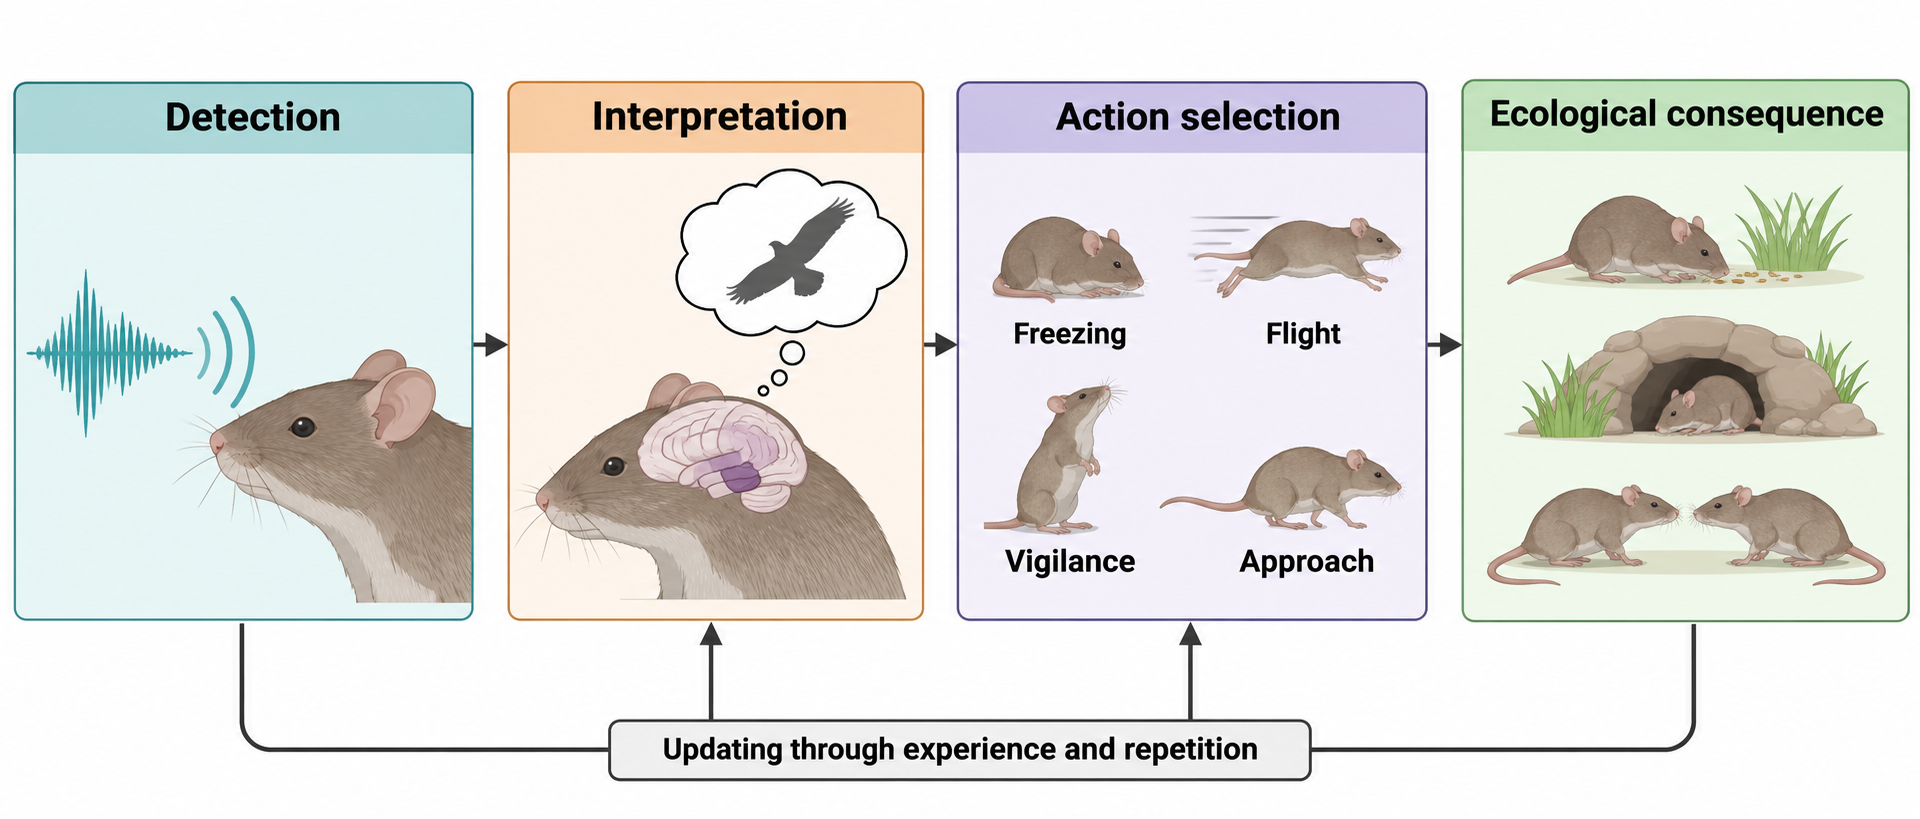
\includegraphics[width=\textwidth]{fig1_framework_placeholder.png}
  \caption{Receiver-centered conceptual model of acoustic significance (schematic). Acoustic information is interpreted in light of experience and source reliability; action depends on ecological state and decision costs; outcomes and repetition update subsequent interpretation. A parallel route links detection directly to action selection, because abrupt or looming sounds can trigger startle, freezing, or flight without learned interpretation (\secref{sec:mechanisms-midbrain}). This is not a strictly serial pathway.}
  \label{fig:framework}
\end{figure}

\subsection{Theory that frames when to respond---but not which sound}
\label{sec:intro-theory}

Functional theory explains \emph{when} receivers should respond. Threat-sensitive avoidance and the economics of escape predict that the strength and type of response should scale with assessed risk and with the relative costs of fleeing and staying \citep{Helfman1989,YdenbergDill1986}. Gray squirrels farther from refuge flee earlier from an approaching visual threat \citep{DillHoutman1989}, a spatial logic that acoustic studies rarely measure. The predation risk allocation hypothesis predicts that vigilance per high-risk period should fall when such periods are frequent \citep{LimaBednekoff1999}; it has not been tested with acoustic cues in rodents (\secref{sec:persistence}). These frameworks motivate the questions developed below. They do not identify which acoustic structures carry significance.

\subsection{Scope and contribution}
\label{sec:intro-scope}

The review concerns \textbf{rodents as receivers}: of conspecific alarm, distress, and social calls; of heterospecific alarms and safety cues; of predator vocalizations played to prey; and, as a contrast, of rat 50-kHz calls, which attract rather than alarm and so constrain any claim that meaningful natural sounds are uniformly threatening. How predators respond to rodent calls lies outside this scope. Visual and multisensory paradigms appear only where needed to delimit an acoustic finding. We do not survey vocal production or applications.

Throughout, we distinguish \textbf{empirical results}, \textbf{theoretical interpretation}, and \textbf{open hypotheses}. The contribution is a synthesis across systems of how acoustic structure, receiver history, ecological context, and updating jointly determine response, organized around three recurring demands on the receiver. It is not a demonstrated unified mechanism, and not a guide to choosing playback stimuli.

\secref{sec:features} asks what information rodents extract from sound. \secref{sec:mechanisms} follows that information into the neural and physiological systems that support, and sometimes dissociate, discrimination, valuation, defense, and changes in body state. \secref{sec:action} compares how ecological and laboratory receivers select actions, and what defensive circuits suggest about field behavior. \secref{sec:persistence} treats updating with experience and repetition. \secref{sec:account} develops an integrated account built on three recurring demands: responding rapidly to salient sounds, learning what sounds predict, and selecting actions according to context and cost. \secref{sec:outlook} identifies outstanding questions. Representative findings are summarized in \tabref{tab:comparison}, with detailed comparisons in \stabref{tab:comparison-supp}{1} and a study-level matrix in \stabref{tab:evidence-supp}{2}.
